\documentclass[14,fleqn]{article}
\usepackage{amsmath}
\usepackage{amssymb}
\usepackage[top=.5 in,left=.5 in,right=.5 in,bottom=.5 in]{geometry}
\usepackage{enumerate}
\usepackage{ mathrsfs }
\usepackage{graphicx}
\usepackage{pgf,tikz}
\usepackage{mathrsfs}
\usepackage{gensymb}
\usepackage{venndiagram}
\usepackage{enumitem}
\usetikzlibrary{arrows}

\pagenumbering{gobble}

\setlength{\parindent}{0 pt}
\setlength{\parskip}{1 ex}

\newcommand{\lcm}{\textnormal{lcm}}
\newcommand{\norm}{\triangleabove right}
\newcommand{\bfm}[1]{$\boldsymbol{#1}$}
\newcommand{\Z}{\ensuremath{\mathbb{Z}}}
\newcommand{\R}{\ensuremath{\mathbb{R}}}
\newcommand{\C}{\ensuremath{\mathbb{C}}}
\renewcommand{\wedge}[1]{\ensuremath{\langle #1 \rangle}}
\newcommand{\infsum}[1]{\ensuremath{\sum_{n=#1}^\infty}}
\newcommand{\defn}[1]{\textbf{\underline{#1}}}
\newcommand{\var}{\ensuremath{\mathrm{Var}}}

%\begin{venndiagram3sets}[labelA=$S$,labelB=$T$,labelC=$U$]
%	\fillA
%	\fillOnlyC
%\end{venndiagram3sets}\\

%\begin{venndiagram2sets}[labelA=$S$,labelB=$T$]
%	\fillNotA
%	\fillNotB
%	\setpostvennhook{
%		\draw[] (labelAB) ++(0,-2.1) node {\raisebox{0pt}[0pt][0pt]{$(S\cap T)'$}};
%	}
%\end{venndiagram2sets}\\

\begin{document}
\section{Section 8.1: Markov Processes}

In real life experiments can be incredibly complicated. But there is one example which is fairly common and useful. Sometimes we have a sequence of experiments where the outcome of each depends only on the results of the previous experiment. Such a sequence of experiments is called a \defn{Markov Process}.

Examples:
\begin{itemize}
	\item A patient is being treated and their blood pressure is monitored. Each day their blood pressure is recored as low, normal, or high and they are treated accordingly.
	\item At UVA students can either be fine academically, be on academic probation, or suspension. Their academic status depends on their last two semesters.
	\item If we have a game with no draws, then each position is either a player 1 win or a player 2 win, and this only depends on the current position of the game.
\end{itemize}

When we have a Markov Process, we assume the experiment is performed at regular intervals, and the possible outcomes are always the same. These outcomes are called \defn{states}. The outcome of the current experiment is called the \defn{current state}. We can describe the outcomes of the experiments with tree diagrams or, even better, state diagrams.

Example: Let's consider the blood pressure example from before. We have the following probabilities for moving between states\\
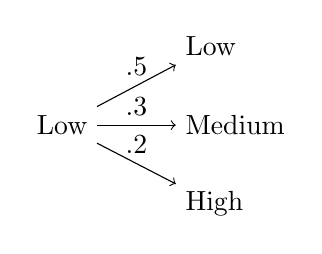
\begin{tikzpicture}
	\node[left] (A) at (0,0) {Low};
	\node[right] (B) at (1,1) {Low};
	\node[right] (C) at (1,0) {Medium};
	\node[right] (D) at (1,-1) {High};
	\draw[->] (A)--(B) node[midway,above] {.5};
	\draw[->] (A)--(C) node[midway,above] {.3};
	\draw[->] (A)--(D) node[midway,above] {.2};
\end{tikzpicture}
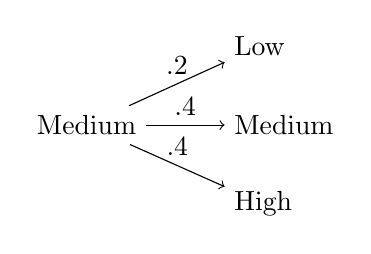
\begin{tikzpicture}
	\node[left] (A) at (0,0) {Medium};
	\node[right] (B) at (1,1) {Low};
	\node[right] (C) at (1,0) {Medium};
	\node[right] (D) at (1,-1) {High};
	\draw[->] (A)--(B) node[midway,above] {.2};
	\draw[->] (A)--(C) node[midway,above] {.4};
	\draw[->] (A)--(D) node[midway,above] {.4};
\end{tikzpicture}
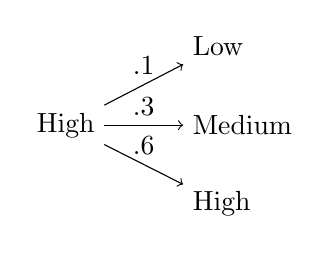
\begin{tikzpicture}
	\node[left] (A) at (0,0) {High};
	\node[right] (B) at (1,1) {Low};
	\node[right] (C) at (1,0) {Medium};
	\node[right] (D) at (1,-1) {High};
	\draw[->] (A)--(B) node[midway,above] {.1};
	\draw[->] (A)--(C) node[midway,above] {.3};
	\draw[->] (A)--(D) node[midway,above] {.6};
\end{tikzpicture}\\
We can also draw a single picture with all of our states on it and every arrow in between. This is called a \defn{state diagram} or \defn{transition diagram}. These help represent our Markof process visually, but there is another representation which is even more useful. Notice how many transition probabilities we need to keep track of. There are 3 states, and 3 probabilites for each state, so we have 9 probabilities, an there is a natural patern of how to right them down. If we have a 3x3 grid we can put the current state at the top, and the next state on the left, and fill in the matrix with the appropriate probabilities.

\begin{tabular}{rrrr}
	&L&M&H\\
	L&.5&.2&.1\\
	M&.3&.4&.3\\
	H&.2&.4&.6\\
\end{tabular}
So what we have is a matrix called the \defn{transition} matrix.

Example: A local library is looking at its membership. It figures that if someone is a member there is an 80\% chance they will renew their membership in the followin year and a 20\% chance they will not. They also assume that if someone is not a member then there is a 10\% chance they will join next year. Write down the transition matrix for this Markof process.\\

Notice 2 things about transition matrices:
\begin{enumerate}
	\item All entries are non-negative
	\item The sum of each column is equal to 1
\end{enumerate}
A matrix satisfying these properties is called a \defn{stochastic matrix}.


Representing the Markov process with a matrix is powerful because we can use matrix operations to help us. Let's look at the library example some more. Suppose that the library initially knows that 60\% of the community is a member of the library and 40\% is not. We can also represent this with a matrix
\[
	\begin{bmatrix}
		0.6\\
		0.4\\
	\end{bmatrix}_0
\]
Where the subscript 0 means that this is the first generation. In general, we can represent our population as an nx1 matrix with entries correspoinding to the proportion of the population in each state. The subscript will represent which generation we are in.\\

Now how do we get the matrix for the first generation. If we let $m_0$ and $n_0$ be the proportion of members and non-members to begin, then we know from the definion of a Markov process that $0.8\cdot m_0$ will renew and $0.2m_0$ will not. Similarly $0.1n_0$ will be come members and $0.9n_0$ will stay non-members. Thus the proportion of members will be $0.8m_0+0.1n_0$ and the proportion of non-members will be $0.2m_0+0.9n_0.$

If we look at the matrices for these transitions we can see that
\[
	\begin{bmatrix}
		0.8&0.1\\
		0.2&0.9
	\end{bmatrix}
	\begin{bmatrix}
		m_0\\
		n_0
	\end{bmatrix}
	=\begin{bmatrix}
		0.8m_0+0.1n_0\\
		0.2m_0+0.9n_0
	\end{bmatrix}
\]
So we can represent transitions with matrix multiplication. If we fill in $m_0$ and $n_0$ then we get the proportion after 1 year. (Actually do the calculation) Notice that it didn't matter what $m_0$ and $n_0$ were, and also notice that after we apply the matrix we still get a distribution matrix. So we can apply the transition matrix to anything we want, including the distribution matrix for the first generation. Let $A$ be the transition matrix and $X_0$ be the distrubtion matrix for generation 0. Then we get the following
\[
	X_1=AX_0\qquad X_2=AX_1=A(AX_0)=A^2X_0\qquad X_3=AX_2=A(A^2X_0)=A^3X_0 \text{ and so on}
\]

We can also consider distribution matrices as probability distributions for each state after a certain number of transitions. This can be useful if we know our first state so our distribution starts out as a 1 in a given place.\\

Example: You have a trip planned with lots of connecting flights. For each flight, it can be either early, on time, or delayed which only depends on the previous flight. If a flight is early then the next flight will be early, on time or delayed with proportions 0.3, 0.5, 0.2 respectively.  If it is on time then the next flight will have probabilities 0.2 0.4 0.4 and if it is delayed then the next flight will have probabilities 0 0.2 0.8. Draw the transition diagram. Find the transition matrix for this Markov process. If the initial flight is equally likely to be early, on time, or delayed, find the distributions for the next 2 generations. If you know your first flight is delayed, find the probability your third flight is early, on time, or delayed.

Interpretation of $A^n.$ If $A$ is the transition matrix, then the entries of $A^n$ have the following meaning. The $ij$ entry of $A^n$ is the probability of the transition from state $j$ to state $i$ after $n$ generations. This can also be seen from appling $A^n$ to the distribution that has $1$ in the $j$ position.

\end{document}
